\section{Materials and methods}

\subsection{Study design}
Study design: Describe overall how the study is structured and why it is that way
% What data processing steps are needed to make a massive accessibility dataset explorable in real-time over the internet?

% What kind of application design should be employed to serve and render geographical data fast enough to enable instantaneous interaction?

% What types of map interaction do people use and prefer in different types of usage scenarios?

% Does map interaction change the map user's perception and understanding of the concept of accessibility? If it does, how?

\subsection{Materials}
Describe the materials used: Travel time matrix files, Collected survey data (and how it was collected), survey participants

\subsection{Methods}
Describe and justify the methods: Data processing, server approach, mapping approach, structure of the survey, analysis of the survey data.

Technical requirements for making the map happen:
\begin{enumerate}
	\item Preprocess the matrix to a mappable format
	\item A back-end to serve the matrix
	\item The web map application
\end{enumerate}

See figure \ref{fig:architechture} for an idea of the architechture.

\begin{figure}[H]
	\centering
	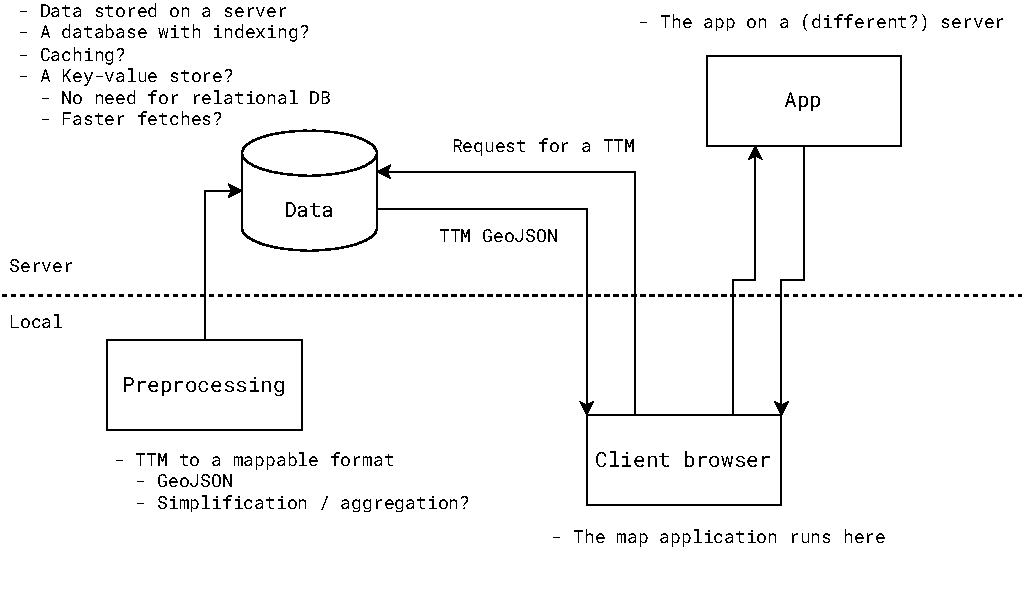
\includegraphics[width=1\textwidth]{images/architechture}
	\caption{Architechture (TTM=travel time matrix)}
	\label{fig:architechture}
\end{figure}

% I see the methods necessary to implement the visualisation belonging to two themes:
% Methods for figuring out how the map should be
% and methods for actually making the map be that way.

% For figuring out what the map should be like,
% I have (hopefully) at this point already formed some ideas from the background section.
% To complement those, and to keep the qualitative aspect of cartography relevant,
% interview(s) will be used alongside the development process.

% When developing the visualisation, the priority should be on the map application.
% However, the development must progress on all components as an iterative process,
% where producing a minimal working state should be the first goal.
% Something that, to some extent, works, makes discussion about the map possible,
% which in turn should keep development progressing towards the right direction.

% It should also be noted that the number of techical options for implementing the map is large.
% Questions such as which mapping library or UI framework to use,
% or how to preprocess the matrix data should be covered here too.
% Depending on the need and extent of comparisons between different technologies,
% some synthesis could be formed about that too.
